\chapter{Revisão Bibliográfica}
	\chapterprecis{Teste, teste}
	
	\section{Laboratório de Operações e Processos - Contextualização}
		O Laboratório de Operações e Processos (LOP) é um dos diversos laboratórios para fins de ensino e pesquisa pertencentes ao Departamento de Engenharia Química da UFMG (DEQ). Ainda existem outros laboratórios vinculados ao departamento cuja finalidade é prestar serviços às comunidades interna e externa à UFMG \footnote{\url{http://www.deq.ufmg.br/departamento/infraestrutura}}.
		
		O LOP possui quatro plantas didáticas: \textbf{explicar aqui brevemente as 4 plantas constituintes do laboratório}
		
		%explicar aqui agora sobre a planta de trocador existente
		O trocador de calor existente no laboratório, cuja imagem pode ser vista na \autoref{fig:lab}, é do tipo tubular. Este sistema, que é fabricado e fornecido pela Universidade de Santa Cecília\footnote{\url{http://cursos.unisanta.br/quimica/laborato/index.html}}, foi adquirido pela UFMG em 2002\footnote{Item 35 do catálogo disponível em: \url{http://cursos.unisanta.br/quimica/laborato/LOU-2016.pdf}}. Originalmente, a planta possui um botão para ligar e desligar bomba e aquecedor simultaneamente, bem como conta com 4 sensores de temperatura, cujos valores são exibidos e display LCDs. A medição de vazão de água quente era inferida através da utilização de uma Calha Parshall\footnote{Funcionamento da Calha Parshall: \url{http://www.dec.ufcg.edu.br/saneamento/PARSHALL.html}}, e a medição de água fria, através da indicação de um rotâmetro\footnote{\url{http://www.sensorsmag.com/components/basics-rotameters}}
		
		\begin{figure}[!htb]
			\centering
			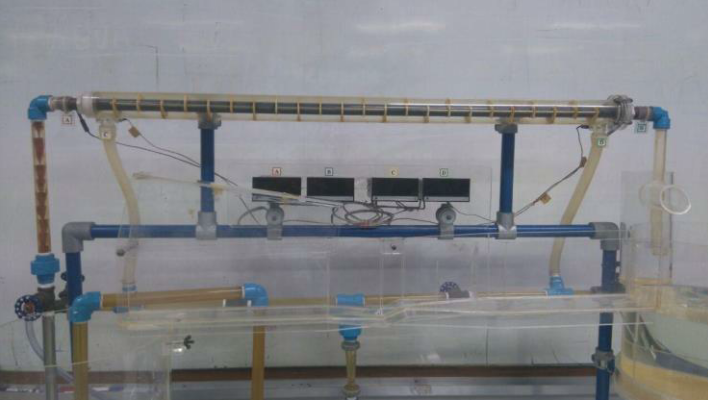
\includegraphics[scale=0.7]{lab}  %pode alterar o tamanho
			\caption{Trocador de Calor presente no LOP.}
			\label{fig:lab}
		\end{figure}

			
		Em 2016, um projeto de modernização desta planta foi iniciado por \cite{luiz2016}.  O projeto consistiu na implementação de um sistema embarcado para operação local e controle da planta. Para alcançar o objetivo, foram feitos os seguintes passos:
		\begin{itemize}
			\item 
			Instalação de quatro novos sensores de temperatura, dois novos sensores de vazão, tornando possível a medição digital das vazões; 2 relés, para o controle do acionamento dos atuadores e um inversor de frequência para controlar a rotação da bomba;
			\item 
			Instalação de um Arduino Due \footnote{\url{https://store.arduino.cc/usa/arduino-due}} para fazer a interface com sensores e atuadores, processar os algoritmos de controle, e exibir os dados em um display LCD. O programa criado no Arduino possibilita a operação em modo automático e manual;
			\item 
			Construção e instalação de um painel para operar e visualizar os dados da planta. Através desse painel é possível selecionar o modo de funcionamento da planta (manual ou automático). Em modo manual, é possível ligar e desligar bomba e aquecedor, bem como controlar a velocidade da bomba e potência do aquecedor. O display LCD permite exibir várias informações como por exemplo valores das temperaturas e vazões, bem como a sintonia dos controladores. Essas informações não conseguem ser expostas ao mesmo tempo para o usuário, portanto um sistema de navegação foi implementado no Arduino. O esboço do painel elaborado é mostrado na \autoref{fig:painel}.
		\end{itemize}
			
			\begin{figure}[!htb]	
				%\centering
				\captionsetup{justification=centering}
				\begin{center}
					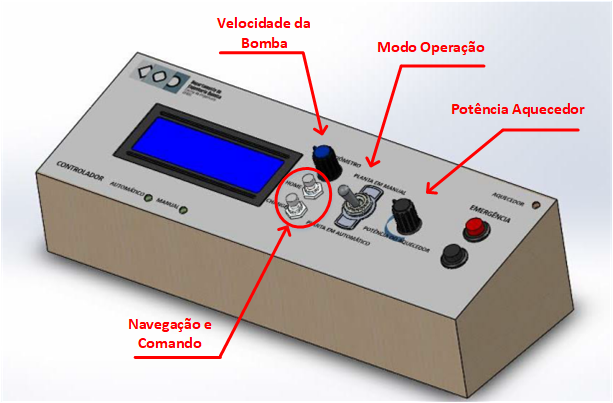
\includegraphics[scale=0.6]{painel}  %pode alterar o tamanho
					\caption[Painel instalado na planta de trocador de calor]{\label{fig:painel}Painel instalado na planta de trocador de calor. \\Adaptado de \cite{luiz2016}}
				\end{center}		
			\end{figure}
		
			A Arquitetura do sistema finalizado é exibida na \autoref{fig:arq_atual}. Destaca-se o fato que não foi possível integrar o controle da potência do aquecedor no Arduino, sendo enviado diretamente do painel. Apesar de previsto no projeto, nenhum algoritmo para controle em malha fechada foi programado.
		
			\begin{figure}[!htb]	
				%\centering
				\captionsetup{justification=centering}
				\begin{center}
					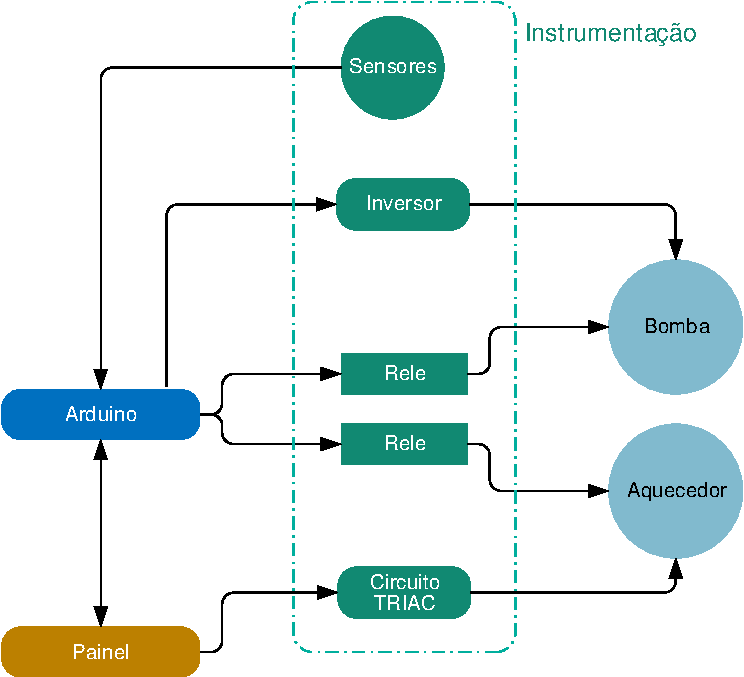
\includegraphics[scale=0.8]{arq_atual}  %pode alterar o tamanho
					\caption[Arquitetura do sistema instalado]{\label{fig:arq_atual}Arquitetura do sistema instalado}
				\end{center}		
			\end{figure}
		
	
	\section{Tecnologias para Controle e Monitoramento de Processos}
		\label{sec:rev_monitor}
		A seguir são apresentadas algumas tecnologias utilizadas para implementar sistemas de controle e monitoramento de processos.
		
		\subsection{Sistemas SCADA}
		Aplicações SCADA são utilizadas na supervisão e controle de largamente empregadas na indústria em setores como saneamento, energia, metalurgia, manufatura entre outros \cite{pablo2011}. Estes sistemas coletam dados de dispositivos de campo e os concentram em ambientes onde possam ser processados e armazenados. Os operadores podem visualizar esses dados através de interfaces gráficas (IHMs), que ilustram o que está ocorrendo na planta em tempo real. 
		
		A arquitetura de um sistema SCADA é mostrada na \autoref{fig:pc_plc}. Estes sistemas são compostos por componentes que são definidos na literatura de acordo com a contribuição no processo de coleta, processamento e exibição dos dados de uma planta.
		
		\begin{figure}[!htb]	
			%\centering
			\captionsetup{justification=centering}
			\begin{center}
				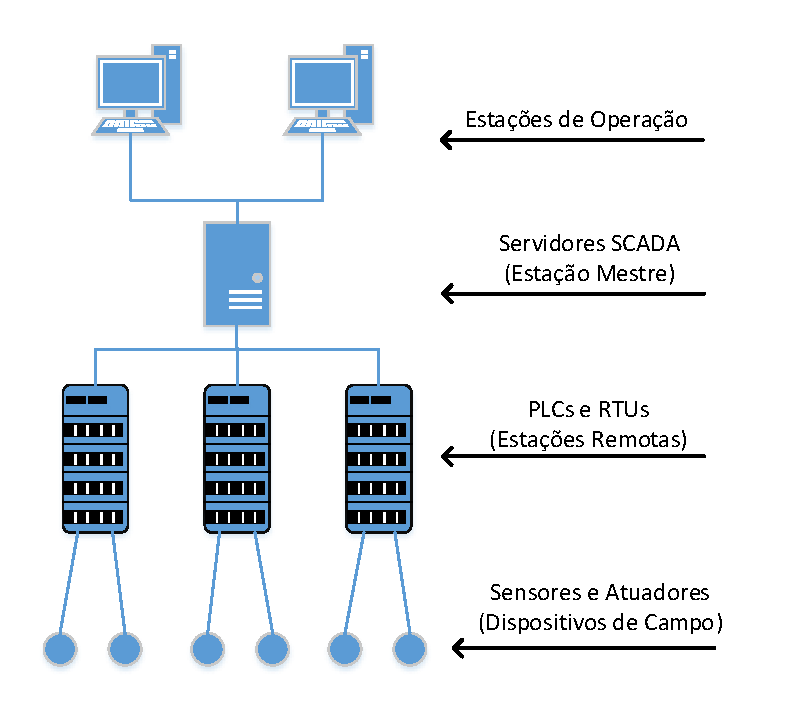
\includegraphics[scale=0.5]{pc_plc}  %pode alterar o tamanho
				\caption[Arquitetura do sistema instalado]{\label{fig:pc_plc}Arquitetura do sistema instalado. Adaptado de \textcite{pablo2011}}
			\end{center}		
		\end{figure}
	
		Dispositivos de campos podem ser entendidos pelos sensores e atuadores. Os sensores medem grandezas físicas do processo. enquanto os atuadores interferem no processo como por exemplo através  acionamento de bombas e válvulas. 
	
		As estações remotas são dispositivos programáveis que possuem a função de fazer a interface entre dispositivos de campo e estações mestre, além de serem dotados de capacidade de executar algoritmos de controle local. Nessa categoria enquadram-se os CLPs e RTUs. Os CLPs surgiram no contexto de chão de fábrica, ou seja, necessidade de programação e menor alcance de comunicação, devida a pequena distância entre os equipamentos. As RTUs surgiram da necessidade de enviar dados de sistemas localizados a grandes distâncias da estação mestre. Contudo, a evolução desses equipamentos tornou difícil a distinção entre eles \cite{bailey2003}.
		
		As estações mestres são o cérebro do sistema. Elas são responsáveis por solicitar dados das estações remotas, processá-los, armazená-los, bem como repassar comandos dos operadores para as estações remotas. As estações mestres são computadores, cuja capacidade depende do porte do projeto. Existem diferentes fabricantes de software que podem ser executados nesses servidores. Alguns fabricantes disponibilizam a opção de separar o processamento em diferentes estações mestres.
		
		As estações de operação executam um software que apresenta uma interface gráfica para o usuário, em que o operador consegue visualizar e interferir no processo através de controles (botões, sliders, etc) disponibilizados pela interface. Em pequenas aplicações, as estações de operação e as estações mestres se encontram nos mesmos computadores.
	
		A comunicação entre estação mestre e remota se dá pela utilização de protocolos industriais abertos como por exemplo Modbus\footnote{\url{http://www.modbus.org/}}, DNP3\footnote{\url{https://www.dnp.org/Default.aspx}}, OPC\footnote{\url{https://opcfoundation.org/about/what-is-opc/}}, entre outros; também há a comunicação através de protocolos proprietários. Este último caso ocorre em sua maioria quando a estação mestre e remota são fornecidos pelo mesmo fabricante.
	
	\subsection{Tecnologia Embarcada}
		Como mencionado no \autoref{cap:introducao}, os sistemas embarcados, estão cada vez mais presentes no setor industrial. \textcite{yu2011}, fazem uma pesquisa sobre os modelos de sistemas embarcados e em quais tipos de aplicações industriais estão sendo utilizados.
		
		Destacam-se a utilização de microcontroladores para executar algoritmos de controle e comunicação com outros sistemas. Um estudo de caso cita o túnel de vento instalado na Universidade de Bradley. A arquitetura do sistema implantado é mostrada na \autoref{fig:lab_view}. Comparando com a arquiteura SCADA descrita anteriormente, os elementos marcados com o número 1, seriam os dispositivos de campo, o microcontrolador (2), seria a estação remota, o PC executando o LabView (3) seria a estação master, e o outro computador seria a estação de visualização (IHM).
		
		\begin{figure}[!htb]	
			%\centering
			\captionsetup{justification=centering}
			\setlength{\belowcaptionskip}{-5pt}
			\begin{center}
				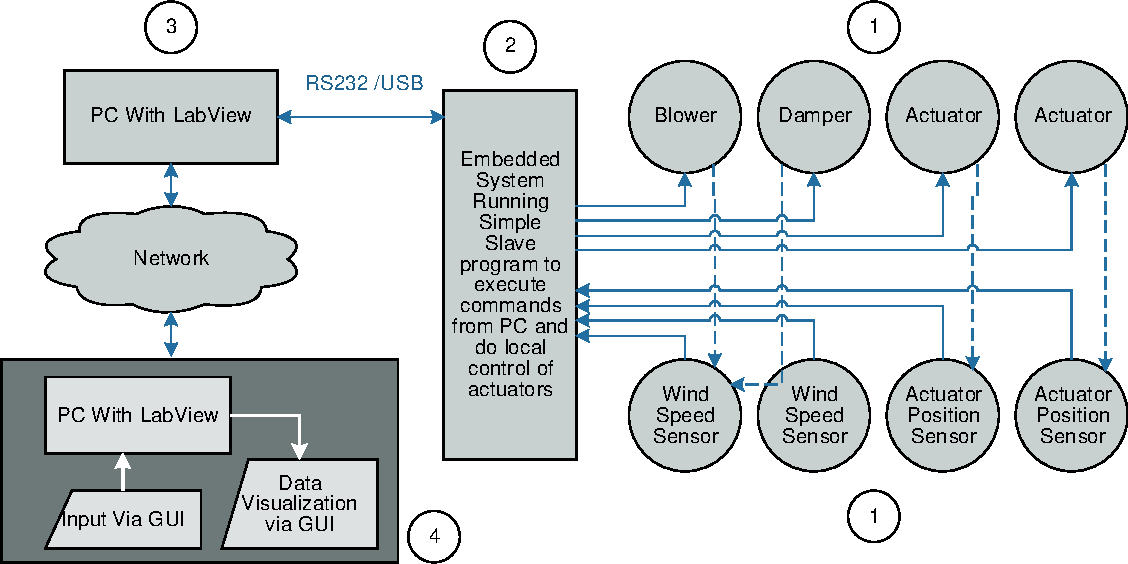
\includegraphics[width=15cm]{lab_view}  %pode alterar o tamanho
				\caption[Exemplo de Sistema com tecnologia embarcada]{\label{fig:lab_view}Exemplo de Sistema com tecnologia embarcada. Adaptado de \textcite{yu2011}}
			\end{center}		
		\end{figure}
	
		O estudo ainda menciona sobre crescimento da utilização de FPGAs\footnote{FPGAs e Microcontroladores: \url{https://www.7pcb.com/blog/fpgas-and-microcontrollers/}} em funções ocupadas pelos microcontroladores, devido a redução dos custos de aquisição dos mesmos, bem como pelas melhorias observadas em relação a capacidade de reconfiguração, o que facilita a sua utilização.
		
		É possível encontrar também diversos trabalhos na literatura que utilizam plataformas de prototipagem eletrônica para conceber projetos de automação para o setor residencial, para plantas de pequeno porte e para projetos na área educacional como plantas didáticas. A portabilidade é uma característica desejada para aplicações desses setores, que também são caracterizadas por possuírem restrições de custo, o que motiva a utilização de hardwares e softwares livres bem como ferramentas multiplataforma.
		
	\subsection{Plataformas de Prototipagem}
		O termo prototipagem rápida designa um conjunto de tecnologias utilizadas para fabricação de objetos físicos diretamente a partir de fontes de dados gerados por sistemas de projeto auxiliado por computador \cite{gorni2001}. A construção do objeto através da agregação de camadas permitem aos projetistas criar protótipos rapidamente.
		
		Este conceito pode ser extrapolado para o desenvolvimento dispositivos eletrônicos. Atualmente no mercado, encontram-se placas baseadas em microcontroladores e microprocessadores que podem se agregar a módulos, construindo assim, um novo produto. Essas placas são reprogramáveis, o que torna o processo de prototipagem rápido e flexível. A seguir serão apresentadas duas das principais placas de prototipagem do mercado.
		
	\subsubsection{Arduino}
		Arduino é uma plataforma eletrônica 	open-source baseado em hardware e sofware flexíveis e fáceis de usar \cite{arduino}. Basicamente a plataforma Arduino consiste em um conjunto de placas
		que possuem um microcontrolador, terminais de entradas e saídas analógicas, digitais e de dados, e uma porta para programação. Como se trata de um hardware livre, é possível que os usuários produzam as próprias placas.
		
		As placas se diferem pela arquitetura do microcontrolador, número de terminais, memória, entre outros. Uma placa pode ter as suas funcionalidades aumentadas através da inserção de Shields, que nada mais são que outras placas fabricadas com propósitos específicos. A placa Arduino UNO\footnote{\url{https://store.arduino.cc/usa/arduino-uno-rev3}} é uma das mais conhecidas, porém existem diversas placas mais poderosas, inclusive que suportam sistema operacional linux, como o Arduino Yun\footnote{\url{https://store.arduino.cc/usa/arduino-yun}}. Como mencionado anteriormente, foi utilizado o Arduino DUE no projeto, que está categorizada como uma das placas mais potentes e com maior número de terminais.
		
		Essa plataforma conta com inúmeras bibliotecas desenvolvidas pela comunidade usuária, que podem ser baixadas diretamente da página do Arduino, ou então disponibilizadas em páginas de compartilhamento de código open-source como o GitHub. A página do Arduino também disponibiliza uma IDE (Integrated Development Environment) para programação da placa. Se o usuário deseja programar em um nível mais baixo, como por exemplo acesso aos registradores internos do Arduino, é possível utilizar o Atmel Studio\footnote{\url{https://www.embarcados.com.br/atmel-studio/}}.
	
	\subsubsection{Raspberry PI}
		Um Raspberry PI é um computador de pequena dimensão (comparável com a dimensão de um cartão de crédito). O objetivo inicial da criação era criar um dispositivo de baixo custo para incentivar a prática de programação em níveis anteriores à graduação. Porém devido ao seu pequeno tamanho, baixo custo e razoável poder de processamento foi sendo adotado em muitos projetos eletrônicos. As placas Rasberry aceitam diversos sistemas operacionais, sendo que o sistema operacional oficial é o Raspian\footnote{\url{https://www.raspberrypi.org/downloads/raspbian}}, uma versão da distribuição Debian/Linux\footnote{\url{https://www.debian.org/}}. Ao longo dos anos, foram lançadas algumas versões das placas, que foram aumentando seu poder de processamento e inserindo mais funcionalidades. Um resumo das características das principais versões lançadas pode ser visto na \autoref{tbl:versoes_rpi}. Uma das grandes vantagens da versão 3, que foi a versão adquirida para o projeto é possuir os módulos Bluetooth e Wifi integrados à placa.
		
		\begin{table}[!htb]
			\centering
			\captionsetup{justification=centering}
			\caption[Comparação entre versões do Raspberry PI]{Comparação entre versões do Raspberry. \\Adaptado de \url{https://en.wikipedia.org/wiki/Raspberry_Pi}}
			\label{tbl:versoes_rpi}
			\def\arraystretch{1.5}
			\begin{tabularx}{\textwidth}{m{2.5 cm}| m{3cm} m{3cm} p{3cm}}
				& \multicolumn{1}{c}{\textbf{Raspberry 1}} & %\textbf{Raspberry 1+} & 
				\multicolumn{1}{c}{\textbf{Raspberry 2}} & \multicolumn{1}{c}{\textbf{Raspberry 3}} \\ \hline
				
				Lançamento & \multicolumn{1}{c}{02/2013} & %\multicolumn{1}{c}{07/2014} &
				\multicolumn{1}{c}{02/2015} & \multicolumn{1}{c}{02/2016} \\
				
				Preço & \multicolumn{1}{c}{\$25} & %\multicolumn{1}{c}{\$25} &
				\multicolumn{1}{c}{\$35} &
				\multicolumn{1}{c}{\$35} \\
				
				Arquitetura & \multicolumn{1}{c}{ARMv6Z} & %\multicolumn{1}{c}{ARMv6Z} &
				\multicolumn{1}{c}{ARMv7-A} &
				\multicolumn{1}{c}{ARMv8-A} \\
				
				CPU & \multicolumn{1}{c}{700Mhz one core} & %\multicolumn{1}{c}{700Mhz one core} &
				\multicolumn{1}{c}{900Mhz quad-core 64bit} &
				\multicolumn{1}{c}{1.2Ghz quad-core 64bit} \\
				
				Memória & \multicolumn{1}{c}{256MB} & 
				%\multicolumn{1}{c}{512MB} &
				\multicolumn{1}{c}{1GB} &
				\multicolumn{1}{c}{1GB} \\
				
				Nº de Portas USB & \multicolumn{1}{c}{1} &
				%\multicolumn{1}{c}{4} &
				\multicolumn{1}{c}{4} &
				\multicolumn{1}{c}{4} \\
				
				Corrente & \multicolumn{1}{c}{300mA} &
				%\multicolumn{1}{p{2cm}}{200mA - 350mA} &
				\multicolumn{1}{c}{220mA - 820mA} &
				\multicolumn{1}{c}{300mA - 1.34A} \\
				
				Wifi Integrado & \multicolumn{1}{c}{Não} & %\multicolumn{1}{c}{Não} &
				\multicolumn{1}{c}{Não} &
				\multicolumn{1}{c}{Sim. 802.11n} \\
				
				Bluetooth Integrado  & \multicolumn{1}{c}{Não} & %\multicolumn{1}{c}{Não} &
				\multicolumn{1}{c}{Não} &
				\multicolumn{1}{c}{Sim. v4.1} \\
				
				\hline
			\end{tabularx}
		\end{table}
	
		O Raspberry possui um conjunto de pinos, que são úteis para realizar comunicação com outros dispositivos através de protocolos como UART, SPI e I2C, bem como enviar e receber informações digitais (nível lógico 0 ou 1) de dispositivos diversos. A \autoref{fig:gpio} mostra os componentes da placa Raspberry Pi 3, bem como uma breve explicação das funcionalidades dos 40 pinos. Observa-se que os pinos que são capazes de realizar comunicação são específicos. Outra informação importante é que os pinos lógicos suportam níveis de tensão até 3.3v, o que difere da tecnologia TTL tradicional, que suporta 5V. Ou seja, caso os pinos sejam submetidos a tensões de 5V, corre-se o risco de danificar a placa.
		
		\begin{figure}[!htb]	
			%\centering
			\captionsetup{justification=centering}
			\setlength{\belowcaptionskip}{-5pt}
			\begin{center}
				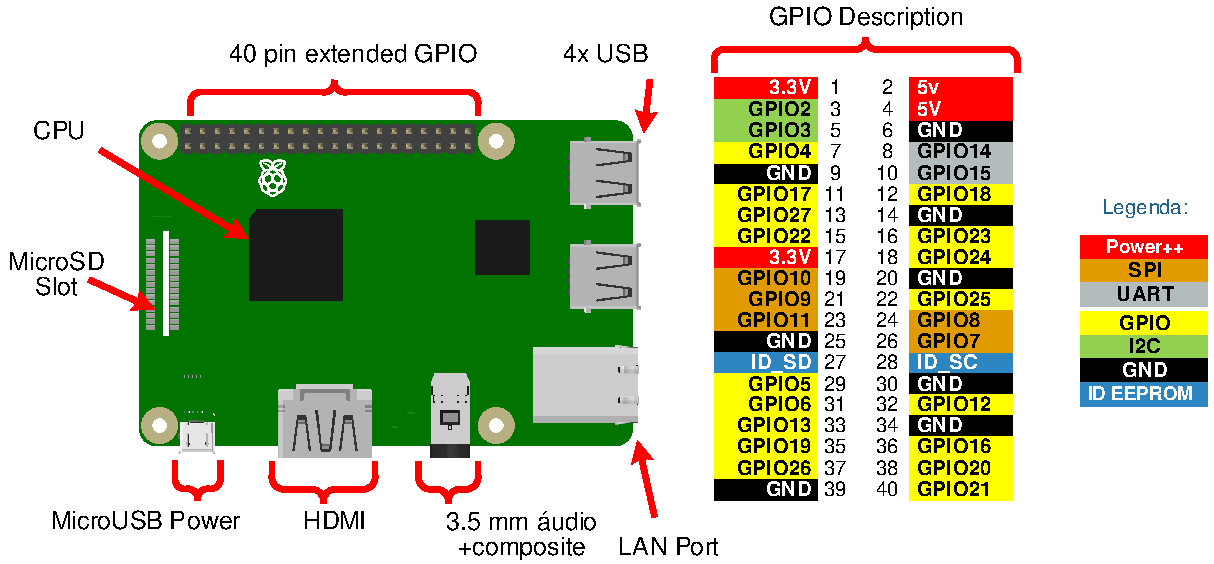
\includegraphics[width=15cm]{rpi_gpio}  %pode alterar o tamanho
				\caption[Composição de um Raspberry PI 3]{\label{fig:gpio}Composição de um Raspberry PI 3}
			\end{center}		
		\end{figure}
	
		\subsubsection{Protocolos de Comunicação}
			Um protocolo de comunicação consiste em um conjunto de regras e convenções criadas para possibilitar a comunicação entre dispositivos. Alguns exemplos de regras existentes em um protocolo: como um dispositivo identifica o outro, quando pode enviar e receber a informação, quanto tempo limite de espera por uma mensagem, entre outros \cite{lucas2016}.
			
			Existem alguns protocolos para estabelecer a comunicação entre Raspberry e Arduino. Basicamente, os protocolos são implementados por bibliotecas, que podem ser utilizadas por Raspberry e Arduino. Como é possível criar softwares em várias linguagens no Raspberry, as bibliotecas a serem utilizadas para esse dispositivo dependem da linguagem de programação utilizada.
			
			Como mostrado na \autoref{fig:gpio}, o Raspberry possui terminais para comunicação SPI, I2C, e UART. Estes protocolos também são suportados pelo Arduino. \textcite{robocore,kevin2015} apresentam um comparativo entre esses protocolos, cujas caracterísitcas estão descritas na \autoref{tbl:comparativo_protocolos}
			
		\begin{table}[!htb]
			\centering
			\captionsetup{justification=centering}
			\caption[Comparação entre SPI I2C e UART.]{Comparação entre SPI I2C e UART. Adaptado de \textcite{robocore}}
			\label{tbl:comparativo_protocolos}
			\def\arraystretch{1.5}
			\begin{tabular}{c c c c c c c}
				Protocolo & Taxa & Sentido & Método & Nº Fios & Tensão & Max \\ 
				& (bps)& Transmissão & & & & dispositivos \\ \hline
				UART & 1200 a 115200 & Full-Duplex & Assíncrono & 2 & 0 a 5V & 1 \\
				SPI & 0 a 10mb & Full-Duplex & Síncrono & 3+N & 0 a 5V & não há \\
				I2C & 100k ou 400k & Half-Duplex & Síncrono & 2 & 0 a 5V & 127 ou 1024 \\
				\hline
			\end{tabular}
		\end{table}
	
		O protocolo SPI possui  a vantagem de o mais rápido entre eles e também ser Full-Duplex. As desvantagens consistem em: aumento do número de fios à medida que o número de dispositivos na rede cresce; alguns dispositivos pode não suportar velocidades muito altas, o que pode causar incompatibilidade na comunicação; é mais suscetível a ruídos.
		
		O protocolo UART possui como vantagem a simplicidade das mensagens envolvidas na comunicação, bem como a sua disponibilidade em diversos dispositivos. Muitas vezes utilizam-se USB e RS-232 para trafegar dados em UART. Como desvantagem destaca-se: limitação em termos de velocidade; ser assíncrono, ou seja é necessário que a taxa de transmissão e recepção seja a mesma para ambos os dispositivos.
		
		O I2C se situa em uma região intermediária entre UART e SPI. É um protocolo síncrono, utiliza-se de apenas 2 fios, e possui uma taxa de transmissão um pouco maior que o UART. Como desvantagem, destaca-se a necessidade de interpretar os pacotes de dados via software, o que pode diminuir a performance de processamento.
		
		\subsubsection{Exemplos de Projetos que utilizaram Plataformas de Prototipagem}
			Encontra-se na literatura, projetos que utilizam placas de prototipagem mencionadas acima, para implementar um sistema de automação de pequenas instalações.
			
			\textcite{lucas2016} implementou a automação de uma planta experimental de um sistema de reaproveitamento de água. O modelo experimental foi construído, instalaram-se sensores e atuadores que se conectam a Arduino. O Arduino se comunica com um Raspberry PI, que possui um sofware SCADA instalado, o Mango automation. Ou seja, essa arquitetura é próxima a de um sistema SCADA tradicional, mostrada na \autoref{fig:pc_plc}. O Arduino faz o papel de uma estação remota, e o Raspberry, de uma estação mestre.
			
			Existe um projeto open-source de um sistema de controle de temperaturas para cervejarias chamado BrewPi \cite{brewpi}. O sistema consiste em um Raspberry PI que comunica com um Arduino, que é encapsulado a uma caixa que possui um display LCD para visualização de informações em modo local. O Arduino implementa algoritmos de controle em malha fechada, bem como possui funcionalidades para ler informações do processo, bem como acionar aquecedor e refrigerador. O Raspberry implementa um WebServer, que disponibiliza os dados do processo para os usuários. Para monitorar o processo, basta um dispositivo que possua um navegador Web. Fazendo um comparativo com a arquitetura SCADA tradicional, o WebServer seria o software SCADA que é executado nas estações mestres, e as estações de operação podem ser representadas por qualquer dispositivo com um navegador Web. Essa arquitetura concede portabilidade à operação, característica desejável a qualquer projeto. A arquitetura do sistema Brewpi é exibida na \autoref{fig:arq_brewpi}. Este projeto é um dos exemplos do crescimento da utilização de sistemas Web para monitoramento e controle de processos.
			
			\begin{figure}[!htb]	
				%\centering
				\captionsetup{justification=centering}
				\begin{center}
					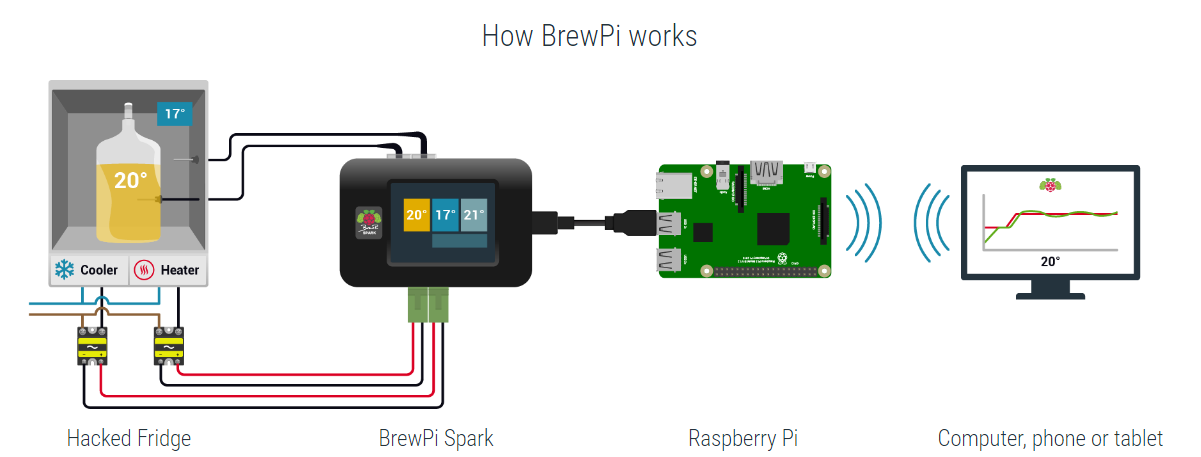
\includegraphics[width=14cm]{arq_brewpi}  %pode alterar o tamanho
					\caption[Arquitetura do sistema BrewPi]{\label{fig:arq_brewpi}Arquitetura do sistema BrewPi. Fonte: \url{https://www.brewpi.com/} }
				\end{center}		
			\end{figure}
		
	\section{Aplicações Web}
		A Web, abreviação do termo \textit{World Wide Web}, que significa em tradução livre ``rede de alcançe mundial'', também conhecida como www, é um sistema distribuído de hipermídia que revolucionou como pessoas organizações e sistemas geram, acessam e compartilham informações \cite{bernes2000}. Foi criada em 1989 por Tim Berners Lee resolver problemas em relação a transmissão e compartilhamento de informações do CERN (Organização Europeia para a pesquisa Nuclear).
		
		Porém o sucesso da Web fez com que a sua utilização não ficasse restrita ao meio acadêmico, sendo utilizada para fins pessoais e comerciais. O crescimento exponencial da Web causou um temor entre a comunidade e pesquisadores da internet, sobre a estabilidade da rede diante da crescente demanda. Diante disso, surgia a necessidade de melhorar a Web em termos de escalonabilidade performance e padronização em relação as aplicações. Em 1994 Berners-Lee fundou a W3C, órgão responsável pela padronização de tecnologias Web, instituição mais importante e reconhecida no mundo sobre o assunto \cite{felipe2008}.
		
		Ao longo dos anos, a Web sofreu transformações, em relação a aplicabilidade e a forma de transmitir informações. Inicialmente, as páginas Web publicavam apenas conteúdo estático, ou seja textos sem muita interatividade. O crescimento da Internet e o aumento da largura de banda fez com que fossem criados sites cada vez mais dinâmicos e interativos, incluindo a participação do internauta na geração de conteúdo, como por exemplo as redes sociais. Atualmente sistemas complexos que antes eram desenvolvidos apenas como aplicativos Desktop, podem ser criados utilizando somente tecnologias Web. A \autoref{fig:evolution_web} e a \autoref{fig:web_apps} exibem um resumo da evolução da web, suas tecnologias e aplicações.
		
		\begin{figure}[!htb]	
			%\centering
			\captionsetup{justification=centering}
			\begin{center}
				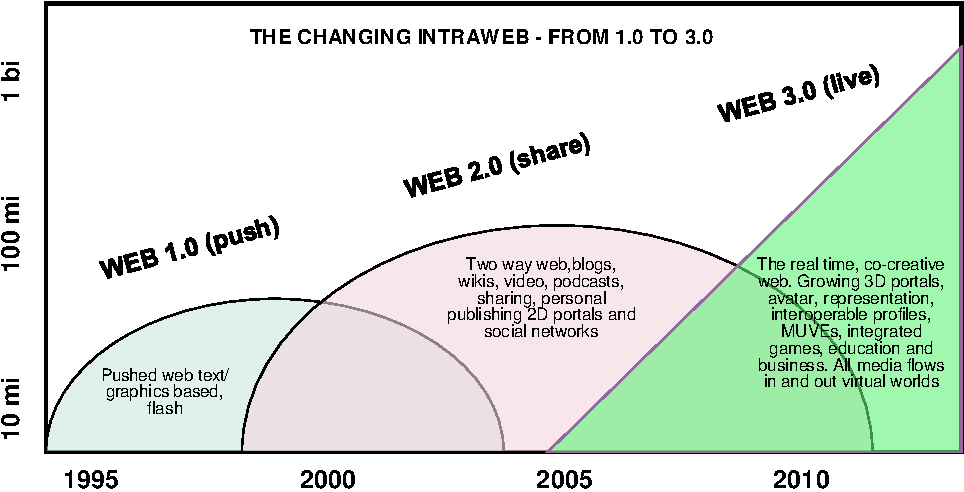
\includegraphics[scale=0.8]{evolution_web}  %pode alterar o tamanho
				\caption[Evolução da Web.]{\label{fig:evolution_web} Evolução da Web. Adaptado de \url{http://www.personalizemedia.com/virtual-worlds-web-30-and-portable-profiles/}}
			\end{center}		
		\end{figure}
	
		\begin{figure}[!htb]	
			%\centering
			\captionsetup{justification=centering}
			\begin{center}
				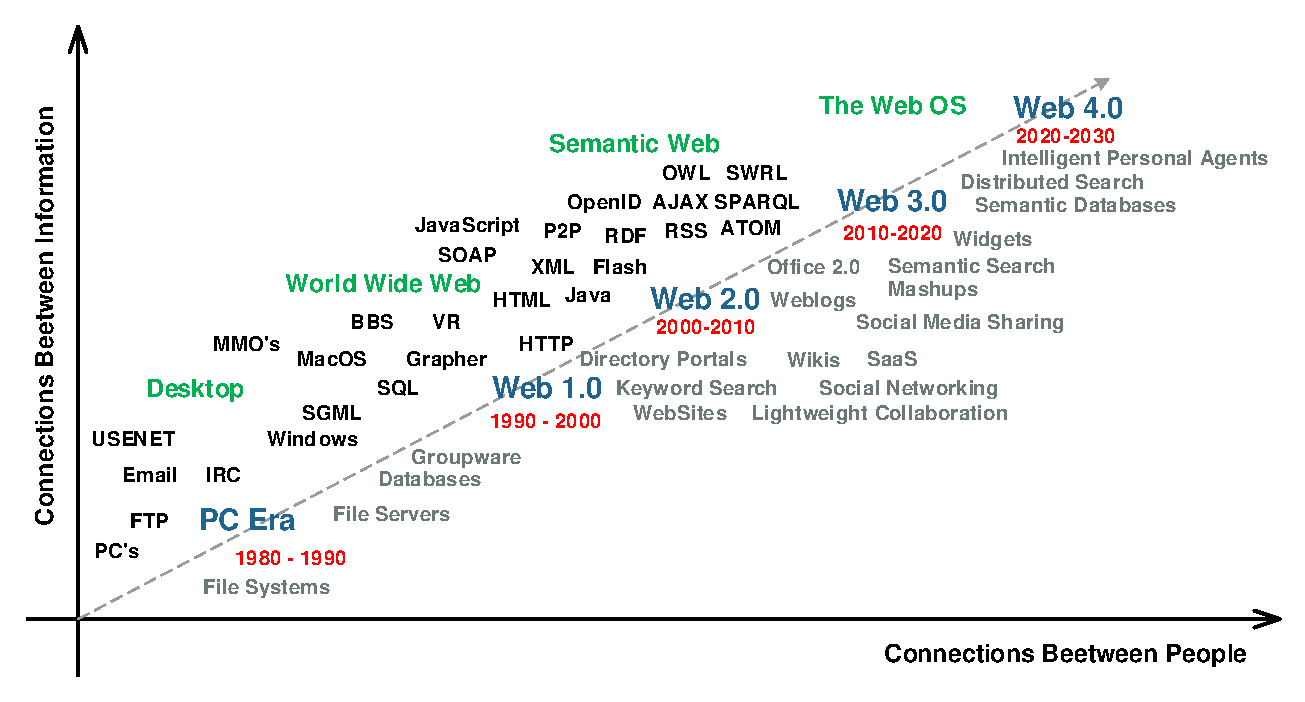
\includegraphics[width=16cm]{web_apps}  %pode alterar o tamanho
				\caption[Evolução da Web. Tecnologias e Aplicações]{\label{fig:web_apps} Evolução da Web. Tecnologias e Aplicações. Adaptado de \url{https://www.prokarma.com/blog/2014/10/16/what-exactly-web-30}}
			\end{center}		
		\end{figure}
		
		Uma aplicação Web tradicional é baseada em estilo cliente-servidor. Basicamente, um servidor oferece serviços e espera por requisições, enviadas por clientes interessados nesses serviços. Ao receberem as requisições, os servidores processam a requisição e enviam uma resposta ao cliente, que é representado por navegadores web. A \autoref{fig:request_response} mostra o fluxo de informações de uma requisição web e a resposta do servidor. As informações trafegam pelo protocolo HTTP\footnote{Especificação HTTP: \url{https://www.ietf.org/rfc/rfc2616.txt}}. Um frame HTTP de requisição possui a estrutura mostrada na \autoref{fig:http_frame}. O método GET é o mais utilizado. Ele possui a função de recuperar algum recurso, que é identificado por sua URL, do servidor Web. Existem outros métodos no protocolo HTTP, como POST, PUT, DELETE, etc \cite{diego2016}. O conteúdo a ser exibido nas páginas é produzido e armazenado em arquivos HTML, que basicamente é um arquivo de texto com marcações. Os navegadores interpretam os arquivos e exibem a página formatada para o usuário.
		
		\begin{figure}[!htb]	
			%\centering
			\captionsetup{justification=centering}
			\begin{center}
				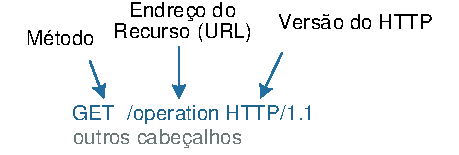
\includegraphics[scale=0.9]{http_frame}  %pode alterar o tamanho
				\caption[Frame de requisição HTTP]{\label{fig:http_frame} Frame de requisição HTTP}
			\end{center}		
		\end{figure}
	
		\begin{figure}[!htb]	
			%\centering
			\captionsetup{justification=centering}
			\begin{center}
				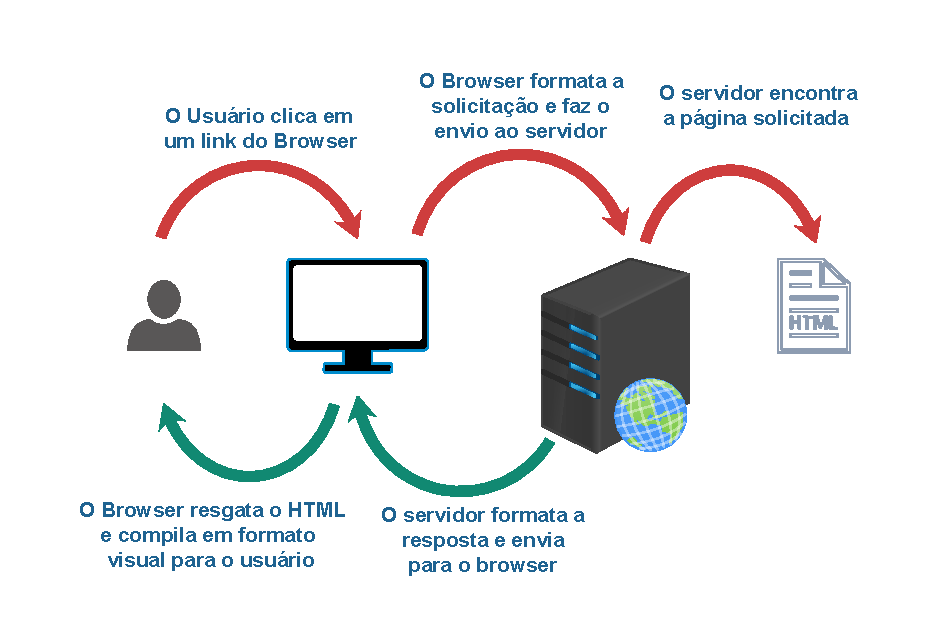
\includegraphics[scale=0.6]{request_response}  %pode alterar o tamanho
				\caption[Funcionamento do sistema requisição resposta.]{\label{fig:request_response} Funcionamento do sistema requisição resposta. Adaptado de \url{https://www.devmedia.com.br/como-funcionam-as-aplicacoes-web/25888}}
			\end{center}		
		\end{figure}
		
	\subsection{Frameworks Web}
		
		